%% The first command in your LaTeX source must be the \documentclass command.
%%
%% Options:
%% twocolumn : Two column layout.
%% hf: enable header and footer.
\documentclass[
% twocolumn,
% hf,
]{ceurart}

%%
%% One can fix some overfulls
\sloppy

%%
%% Minted listings support 
%% Need pygment <http://pygments.org/> <http://pypi.python.org/pypi/Pygments>
\usepackage{listings}
%% auto break lines
\lstset{breaklines=true}


%%%%%%%%%%%%  additional packages  %%%%%
\usepackage{LOA-template}
%%%%%%%%%%%%  -------------------  %%%%%

%%
%% end of the preamble, start of the body of the document source.
\begin{document}

%%
%% Rights management information.
%% CC-BY is default license.
\copyrightyear{2022}
\copyrightclause{Copyright for this paper by its authors.
  Use permitted under Creative Commons License Attribution 4.0
  International (CC BY 4.0).}

%%
%% This command is for the conference information
\conference{\TODO{Woodstock'22: Symposium on the irreproducible science,
  June 07--11, 2022, Woodstock, NY}}

%%
%% The "title" command
\title{A better way to format your document for CEUR-WS}

\tnotemark[1]
\tnotetext[1]{You can use this document as the template for preparing your
  publication. We recommend using the latest version of the ceurart style.}

%%
%% The "author" command and its associated commands are used to define
%% the authors and their affiliations.
\author[1,2]{Dmitry S. Kulyabov}[%
orcid=0000-0002-0877-7063,
email=kulyabov-ds@rudn.ru,
url=https://yamadharma.github.io/,
]
\cormark[1]
\fnmark[1]
\address[1]{Peoples' Friendship University of Russia (RUDN University),
  6 Miklukho-Maklaya St, Moscow, 117198, Russian Federation}
\address[2]{Joint Institute for Nuclear Research,
  6 Joliot-Curie, Dubna, Moscow region, 141980, Russian Federation}

\author[3]{Ilaria Tiddi}[%
orcid=0000-0001-7116-9338,
email=i.tiddi@vu.nl,
url=https://kmitd.github.io/ilaria/,
]
\fnmark[1]
\address[3]{Vrije Universiteit Amsterdam, De Boelelaan 1105, 1081 HV Amsterdam, The Netherlands}

\author[4]{Manfred Jeusfeld}[%
orcid=0000-0002-9421-8566,
email=Manfred.Jeusfeld@acm.org,
url=http://conceptbase.sourceforge.net/mjf/,
]
\fnmark[1]
\address[4]{University of Skövde, Högskolevägen 1, 541 28 Skövde, Sweden}

%% Footnotes
\cortext[1]{Corresponding author.}
\fntext[1]{These authors contributed equally.}

%%
%% The abstract is a short summary of the work to be presented in the
%% article.
\begin{abstract}
  Functional modelling is a well-studied topic in engineering, biology, and other disciplines. 
  In particular, functional modelling is an essential part of describing engineering systems.
  Therefore, research on functionality is of interest for applications.
  In this paper we analyze some typical problems that are encountered when modeling engineering systems, which are intertwined with functional aspects, such as granularity, malfunctioning representation, and permanence of identity.
\end{abstract}

%%
%% Keywords. The author(s) should pick words that accurately describe
%% the work being presented. Separate the keywords with commas.
\begin{keywords}
  Functional modelling \sep
  Functional decomposition \sep
  replacement %% \sep
  %% diacronic identity permanence %\TODO{[?]}
\end{keywords}

%%
%% This command processes the author and affiliation and title
%% information and builds the first part of the formatted document.
\maketitle

%% TODO "theory" --> "ontology"?

\section{Introduction}
    
Functionality is an essential concept in engineering and its use in modeling is widespread. 
Unfortunately, though several theories of functionality have been proposed, no unique treatment has emerged, and some problems persists.
In this papers, we describe some of the problems that current theories face and, building on previous work, we show, using an \TODO{industrial use case as example}, possible ways to tackle them through applied ontology. 

%% introduction & very brief review
\section{Some brief points from the literature}

Functionality is a well-studied topic in engineering \cite{chandrasekaranFunctionalRepresentationDesign1993, umedaFunctionBehaviourStructure1990, hirtz_functional_2002} and ontology \cite{sasajimaFBRLFunctionBehavior1995, TowardAUnifiedDefinition2012}, at least from more then 50 years \cite{collinsFailureExperienceMatrixUseful1976,pahl_engineering_2007} (see also \cite{erdenReviewFunctionModeling2008} for an in-depth review of some aspects of the function-related literature).
We recall very briefly the main characteristics of some theories (or methodologies) of functionality that have been developed in engineering until today.

\begin{itemize}
    \item \textbf{Functional Basis} \cite{hirtz_functional_2002,stone_development_2000}: this methodology consider functions as black-boxes that operate transformations on inputs, producing outputs. The Functional Basis is a vocabulary for functions (e.g., `convert', `branch') and inputs/outputs (called flows, e.g., `pressure', `electric energy'). The vocabulary is organized in three levels of increasing specialisation. A functional model is a graph of boxes and arrows labeled with function and flows terms respectively, which describes the transformations that the flows that enter an engineering system undertake.
    \item \textbf{Functional Representation} \cite{chandrasekaranFunctionalRepresentationDesign1993}: this methodology requires to, first, build a structural model of the system, which is modelled as a set of devices, each one with a set of relevant parameters and input/output ports, and of relations between devices, e.g. the connection between two ports or the containment of one device into another. Then, state variables are attributed to the system and used to determine different system states. Lastly, the system behaviour is represented as a set of state transitions, each one justified either by a `causal process description' (CPD), a `domain law', or a component `function'. CPDs and functions can then be justified by other CPDs or functions, forming a sort of explanation tree. Therefore, in this methodology, functions are justifications for state transitions. Indeed, they can be enriched by stating the starting state, the terminating state, and evental conditions necessary to start the transition.
    \item \textbf{FBRL} \cite{sasajimaFBRLFunctionBehavior1995, kitamuraOntologicalModelDevice2006}: this framework also requires a structural model of the system. This is done through the so-called device ontology, which is similar to the structural models of Functional Representation. Then, a particular class of devices behaviours is selected (\quotes{behavior based on states of the flowing operands at ports of a device}, `operands' being similar to Functional Basis flows). Functions are roles that these behaviours play in the context of the system. The separation between behaviours and functions explains the possibility for a device to have different functions despite having the same behavior (e.g., a heat exchanger can either cool or warm a liquid flowing into one of its port, depending of the system). Moreover, the vocabulary of functional terms (such as `to join') is distinguished from the vocabulary of `way-of-achievement' (such as `welding', which is a possible way to achieve the `to join' function), this vastly reduces the number of functional terms and allows engineers to build domain-specific databases of `way-of-achievements' (while the functions are domain-independent). Finally, to give a teleological explanation of a system some relations between functions, called `meta-functions', are proposed (e.g., the give heat function of the boiler \textit{drives} the rotate shaft function of the turbine). 
\end{itemize}
Several other theories or methodologies exist, but a complete list is outside the scope of this paper. The interested reader can see, for example, \cite{umedaFunctionBehaviourStructure1990,qianFunctionBehaviorStructure1996, zhaoStateBehaviorFunction2019} among others.
In addition, there are also the theories of functionality developed by the ontological-philosophical community, for example \cite{cumminsFunctionalAnalysis1975} or the considerations of the authors of upper ontologies such as \BFO, \GFO, \YAMATO, or \DOLCE (see e.g. \cite{spearFunctionsBasicFormal2016, herreGeneralFormalOntology2006, sasajimaFBRLFunctionBehavior1995, borgoFormalOntologicalPerspective2009}, respectively)\footnote{Note that some of these works, \BFO and \GFO especially, are partially or completely focused on developing functional theories for biology and not for engineering.}

Theories of functionality attempts to solve practical and theoretical problems, and to achieve some desiderata.
Classical lists of general desiderata are \cite{vermaasAscribingFunctionsTechnical2003,artigaReorganizingOrganizationalAccounts2011}, among others. In order to adapt them to this work we take only a subset of items and we modify them slightly:
\begin{itemize}
    \item \textbf{Distinction between different types of function.} In philosophy, the classical example is proper versus accidental (e.g., using a hammer to nail something versus using the same hammer as a door stopper), but technical distinction used in engineering could be main function versus secondary function versus safety function (e.g., a system of gears has the main function of transferring rotational movement and/or varying the angular velocity. In order to maintain this function a designer will have to implement some cleaning/lubrication system with the secondary function of maintaining the correct motion between the gears and preventing wear. Finally, if, say, the gears are such that there is the danger for the workers to get impinged within them, then a system with some safety function should be present, as physical barriers between the workers and the gears or automated stoppage systems). Not all authors use such distinctions, but they are neverthelless quite widespread \TODO{citare almeno i tedeschi[?]}.
    \item \textbf{Accounting for malfunctions.} It should be possible to describe the case that an artifact has a function even if it does not work (at least not currently). Notice that this desideratum is essential, especially in the maintenance domain, which revolves around the possibility for an object to malfunction.
    \item \textbf{Describing the link between function of an object and its physical properties.} That is, every function in an object shoul be realized by virtue of necessary and/or sufficient set of physical properties (e.g., we would not be able to use the hammer as a door stopper if it were very light).
    \item Accounting for innovation. The theory should be able to represent functions of newly invented artifacts and the innovation in the functionality of existing artifacts. \TODO{remove?}
    \item \textbf{Teleology.} The theory of function should help the process of explaining the working of a system. 
\end{itemize}
The previous list is made of general principles, while, coming to theory of functions devised to help engineers with their tasks, such as design, diagnosis, or troubleshooting, we find another classical desiderata: `no function in structure' principle \cite{kleer_qualitative_1984}. The original formulation of De Kleer is \quotes{the laws of the parts of the device may not presume the functioning of the whole} \cite{kleer_qualitative_1984}. This principle has the goal of making description of devices independent of any particular application, to facilitate modularity. Subsequent critics were moved to the applicability of such principle \cite{keunekeExploringNoFunctionInStructurePrinciple1989}. \TODO{[...] [Chanderasandekar e mode of deployment].} We want to focus on a derivative aspect of the `no function in structure' priciple: 
\begin{itemize}
    \item \textbf{No function in structure?} What is the relation between functionality of an object and the system(s) in which that object can operate? For example, does a battery have a function independently of the particular system(s) in which it could be inserted, or it has a function only when part of a system? %what is the relation between . Information about functionality and information about structure of an engineering system should refer to indipendent background knowledge (they should refer to different `modules', using language mutuated from knowledge engineering \todo{comp. science?}). This priciple has the goal of allo
    \item 
\end{itemize}
Anoter recurring problem is the one of functional decomposition.
The last point raise the issue of the correct representation of engineering artifact from an ontological 
To these desiderata we add some classical
To those points, we concern

\begin{itemize}
    \item Functional decomposition
\end{itemize}

Functional decomposition is essential, because of multiple reasons. We lists some of those in the following (some points refers to the structural hierarchy and not to the functional one, but, if we assume that some relation exists between the physical components of a system and its functions, they translate to the functional hyerarchy as well):
\begin{itemize}
    \item Accounting for different viewpoints. Different operations carried out on a product during the various step of its lifecycle require different point of views about the product. Those viewpoints may differ also due to the level of granularity they focus on, for example, during assembly of a machine, a car say, it may be very important for the workers to know where each screw goes and what kind of washer is required. On the other hand, during maintenance, it may happen that, if a part of the car is malfunctioning, it is simply replaced as a whole, and no diagnostic is carried out to determine what was wrong within that part, because it would be too costly in time and money, even if that part was assemblied by the same company that is carrying out maintenance. 
    \item Simplifying the management of complex systems. Engineered systems can be extremely complex, and when that happens it would be very difficult to manage them using the a fixed level of granularity. This is because that level would necessarily be the atomic one, otherwise some information would be lost, but this would be akin to treat a complex system, say a car, as a list of screws, bolts, pipes, metal plates and pieces of various shapes, etcetera, which would be untenable.
    \item Reasoning about engineering systems. Human reasoning about engineering systems often requires jumping between differentlevels of granularities. For example, the german school of sytematic design \cite{pahl_engineering_2007} explicitly describes the design process as the developement of a functional hierarchy (`functiostrukture') starting from the highest level of granularity (the main function the product to be designed should satisfy) going down to `smaller' functions until one reaches a point that can be readily translated to an assembly of physical items (`embodyment' of the functions). Analogously, a common way for technicians to troubleshoot a malfunctioning system is to produce a chain of parts, each one `containing' the malfunction and `smaller' then the preceeding part. The method used to isolate the next part of the sequence vary, but it could very well be based on function of the part (e.g., if a laptop is not playing music correctly the problem will be -- among other possibilities -- in its speakers; if, more precisely, the music is played always too softly, the problem will be in the amplifying circuit within the speakers, etc.)
    \item Allowing scalability of applications. Suppose that one were to implement either a proof of concept or a production-ready\TODO{[?]} application (also) based on the theory of functionality. If the proof of concept has to be translated into a production-ready application, or if the 
\end{itemize}

The previous points highlight the importance of functional decomposition and, more in general, of granularity in functional or structural models. 
Since granularity is an important concept forthis paper, we shall precise what we mean, in this paper, when using such word.

\bflist
\item[\mydf{}]
    Given any binary relation $R$ in some domain of discourse, whose transitive closure is a (strict or non-strict) partial order, we say that an element of the domain $x$ is at lower (or finer, or, informally, `smaller') granularity level than the element $y$, with respect to the relation $R$, if and only if there exist some elements $x_1$, $x_2$, \dots, $x_n$ such that $R(x,x_1)$, $R(x_1,x_2)$, \dots, $R(x_n,x)$. 
    Additionally, saying that $x$ is at a lower (finer, smaller) granularity level than $y$, is the same as sayng that $y$ is at a higher (coarser, bigger) granularity level\footnote{The constrain on the transitive closure prevents unwanted scenarios such as domain elements which are, at the same time, both at higher and lower granularity level of other elements}.
    Finally, `zooming in' (or `zooming out') from an element, or moving to a finer (coarser) level of granularity are expressions meaning that, given some domain element, we consider a set of elements that are ar a finer (coarser) granularity level than the starting element.
\eflist
An immediate consequence of this definition is that we can `zoom in' or `zoom out' to a new granularity level along different relations. For example, suppose that we want to model a combustion engine. Simplifying, we take the engine as composed by three parts: the carburetor (that mixes the fuel with air), the intake manifold (distributes the air/fuel mix to the cilynders), and the cylinder group. Then, from the point of view of the mereological part-of relation we have a tree structure, where the root is the engine (as a whole), which has three leaves attached (the carburetor, the manifold, and the cylinder group); and we can zoom in or out over this tree structure. Additionally, if a taxonomy\footnote{That is, a directed acyclic graph (usually a tree, but sometimes one accounts fo multiple inheritance) between classes of entities whose edges represent the subsumption (is-a) relation.} is present, it could be used to zoom in or out over the is-a relation. Therefore, granularity could be varied along different dimensions, see Figure \ref{fig:2-ways-granularity-table-new-new} for an exemplification. 

In the very same way, if we have a taxonomy of function-types, together with a relation of aggregation/decomposition of some kind between functions, we can vary the granularity of any functional model along these two different relations. See Figure \ref{fig:2-ways-granularity-table-function}, which uses the Functional Basis methodology for representing functions, for an exemplification.

\begin{figure}
    \centering
    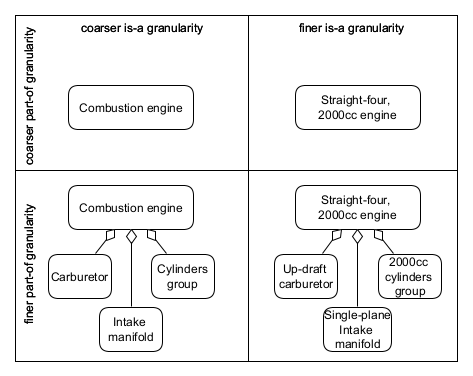
\includegraphics[width=\textwidth]{2-ways-granularity-table-new-new.PNG}
    \caption{\label{fig:2-ways-granularity-table-new-new}A simplified structural model of a combustion engine. Starting from the engine as a whole one can go towards a finer mereological-granularity and find out that the engine is made of three components; going towards a finer subsumption-granularity one can find out that the engine is not just an instance of any combustion engine, but has additional properties (in this case the number, location, and volume of the cylinders), and the same holds fro the engine parts.}
\end{figure}

\begin{figure}
    \centering
    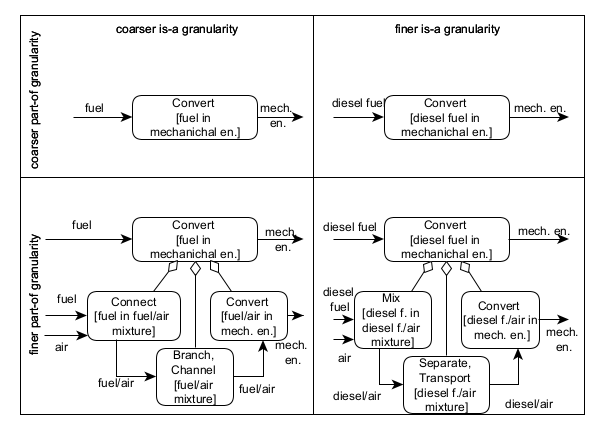
\includegraphics[width=\textwidth]{2-ways-granularity-table-functions.png}
    \caption{\label{fig:2-ways-granularity-table-function}A simplified functional model of a combustion engine using the Functional Basis methodology. For simplicity, we refer to thestructure in Figure \ref{fig:2-ways-granularity-table-new-new} and assume that each part of a system has a function. Using the Functional Basis vocabulary, the function of the engine could converting fuel into mechanical energy, while the function of carburetor is to mix fuel and air, and so on for the other components. In this case, zooming in on the aggregation relation means decomposing the current function, while zooming in on the is-a relation is achieved by moving on a lower level of the functions vocabulary (e.g, from `connect' to `mix'), as well as using more precise terms for the flows.}
\end{figure}

How does it look like a theory of functionality for the engineering domain?
\begin{itemize}
    \item It is part of an 
\end{itemize}

\subsection{The problem of diacronic identity of sytems components}
Another classical problem that arises when attempting to model engineering systems is the replacement problem \cite{guarinoArtefactualSystemsMissing2014},  \cite[Chapter 14]{westDevelopingHighQuality2011}. Therefore, a theory of functions (possibly in conjunction with the other theories used to model non-functional aspects) should help to explain diacronic permanence of identity of systems components:
\begin{itemize}
    \item \textbf{The replacement problem.} In maintenance, the replacement of a malfunctioning component with another is common occurrence. Thus, it happens frequently that a (sub)system has many or even all of its parts changed, but the (sub)system stays the same. This should be explained. This is \TODO{reference to hodkiewicz?}.
\end{itemize} 



--------------------------------

In previous works we have explored the [...]

A subdivisition 

If functions are conceptualized as dispositions then one can account for malfunctioning by saying that, for example, dispositions can be either realized, this is the case of an artifact working as intended, or not, for example when an artifact malfunctions. But, if the artifact is replaced, since the disposition inheres in it, the artifact function should be removed from the system and when another artifact is installed, a different function would be `brought in' the system. In this case we would only be able to state that the two different functions belong to the same type.

Additionally, if we want to model functional locations in theory, whatever they are, surely we want to attribute to them a function (the alternative, function-less functional locations, seems weird). Then, functional locations would survive replacement of constituting components, while the corresponding functions would not. In particular, between replacements (that is, during occurrences of the missing component problem), there would be no constituting component, thus no function.

In conclusion, the conceptualisation of functions as entities inhering to physical objects does not explain well diacronic identity peculiarities of engineering systems.
An obvious idea to solve this issue is to introduce in the domain of discourse `stable' \cite{compagnoComparingOntologicalAlternatives2021}, `conventional' \cite{guarinoArtefactualSystemsMissing2014}, or simply `system' \cite{westDevelopingHighQuality2011} \TODO{attenzione: per West functional objects != system component != role} components, which are entities such that survive replacement as a defining property.   
This is the way ISO 15926 solves this problem, in this case a category of objects is introduced, called `functional objects'. Indeed, in the current working draft is not explicitly stated, but is strongly entailed that functional location is synonymous with functional object [see Figure G.bla.bla].  

Then, functional objects are associated to a function, and survive replacement of the physical objects installed in their place, which are reduced to constituent.

An obvious parallel for functional objects in a plant/machine are the various roles of a sports team. For instance, if a soccer team requires one goalkeer, three strikers, etc., then those roles can be played by different people at different time and sometimes could even being vacant.

From an ontological point of view it is tempting to identify such functional objects/functional locations as roles. Indeed, in \cite{guarinoFormalOntologyProperties2000} role are characterized as an classes which are antirigd (that is, role-players are not necessarily so) and existentially-dependent (that is, when a role exists another entity must exist, e.g. for a goalkeeper-role to exists a soccer team must exist). These two meta-properties are satisfied by functiontional locations, sice their constituents can be missing or replaced, and functional objects existentially-depend on the systems they are part of (`functionalPartOf' using ISO 15926 language).

Assuming that a 

What is a functional location?
`[In the context of] Plant Maintenance, 
An organizational unit in Logistics that structures the maintenance objects of a company according to functional, process-oriented, or spatial criteria. A functional location represents the place at which a maintenance task is performed.' Notice that, despite the name, the spatial criteria is only one possible criteria for identifying the functional location.
\url{https://help.sap.com/glossary/?locale=en-US&term=functional%2520location} accessed May 2022.


`ISO 15926-14 includes terms for defining restrictions identified in the design phase and terms for the transition from design to procurement. This includes in particular class terms for physical objects, systems, functions and functional objects. 

Using these terms one can capture the evolution of functional objects from an early design phase to the functional locations of tag numbers and capture the distinction between a tag number and a physical object installed at the tag. This feature is exploited in the modelling patterns for lifecycle information.' --page 11

`The starting point is a system s, with functional parts a and b represented by the object property functionalPartOf. Both the system s and its functional parts a and b are classified as FunctionalObject. A functional object could be a tag, or an object identified in the design process at a point before tags are introduced.' --page 60

`An important point is that the breakdown structure of the physical objects may be very different from the system breakdown structure captured by the object property functionalPartOf. The physical breakdown structure is not illustrated, but could be captured by part/whole properties, e.g., arrangedPartOf.' --page 61

`The story begins with the creation of a functional object that fulfills the need for pumping. The object is then associated with Function Requirements (FR) specifying such details as rated power, etc. Next, the location for the object is specified as well as the Component Type (CT) and a Product Specification (PS) is given. Once the specifications are in place, an actual motor, i.e. a physical object, is installed and, later, replaced by another motor as part of a maintenance policy.' -- page 65

`Class: lis:System Annotations: rdfs:comment "A system is a complex of functional parts working together. Each part contributes to the realisation of the system's function (though not necessarily every part in every performance of the system).", rdfs:label "System", skos:note "A functional location that does not itself have functional parts is not a system.",' --annex F

functional locations are implicitly equiparated to functional objects, see Figure G.5.3.

`Class: lis:FunctionalObject Annotations: rdfs:comment "A functional object is part of a system, and has a function whose realisation contributes to the performance of the system as a whole.", rdfs:label "FunctionalObject", skos:example "An item on a Process Flow Diagram (PFD) or Process and Instrumentation Diagram (P\&ID) should be classified as a FunctionalObject.", skos:note "A class of artefacts such as Pump is not a subclass of FunctionalObject: a pump that is not in service is not part of a system. However, an individual functional location should in general be given some high-level artefact classification in addition to its description as part of a system.", skos:prefLabel "FunctionalObject" SubClassOf: lis:Object, lis:functionalPartOf some lis:System, lis:hasFunction some lis:Function Every object in an industrial plant is there for a purpose, and the objects are arranged into systems of “functional objects”. Plant design assigns one or more functions to each functional object'--page 20[10]

%% use case application

\paragraph*{The semantic of tags}




%% conclusions

\bibliography{biblio-funzioni}

\end{document}